\section{Grundlagen}

\subsection{Machine-Learning-Modelle}\label{sec: Machine Learning Modelle}
In diesem Kapitel werden die verschiedenen Machine-Learning-Modelle beschrieben, die in dieser Studienarbeit verwendet werden. Es wird erläutert, wie jedes Modell funktioniert und in welchen Anwendungsbereichen es typischerweise zum Einsatz kommt.

\subsubsection{Lineare Regression}\label{sec: Linear Regression}
Die lineare Regression ist ein statistisches Verfahren, das eine lineare Beziehung zwischen einer abhängigen Variable (y) und einer oder mehreren unabhängigen Variablen (X) modelliert. Das Modell findet häufig Anwendung in Vorhersageszenarien, beispielsweise zur Prognose von Preisen, Verkaufszahlen oder Temperaturwerten anhand vorhandener Daten. 

Die lineare Beziehung wird durch die Gleichung \(y(x) = mx + b\) beschrieben, wobei \(m\) die Steigung und \(b\) der y-Achsenabschnitt ist. Ziel ist es, die Parameter \(m\) und \(b\) so zu schätzen, dass sie die beste Anpassung an die Daten bieten. 

Zur Bewertung der Modellgenauigkeit wird eine Verlustfunktion, wie der Mean Squared Error (MSE), herangezogen. Das Training des Modells erfolgt durch Anpassung der Parameter \(m\) und \(b\), um den Verlust zu minimieren.

\autoref{fig: Lineare Regression} illustriert ein Beispiel für eine lineare Regression, bei der eine Gerade so durch die Datenpunkte gelegt wird, dass der Gesamtabstand zu diesen Punkten minimal ist. Wird ein neuer Wert \(x_{\text{new}}\) hinzugefügt, kann der zugehörige y-Wert (\(y_{\text{new}}\)) durch Einsetzen von \(x_{\text{new}}\) in die Gleichung prognostiziert werden.

\begin{figure}[H]
	\centering
	\begin{tikzpicture}
		\node [anchor=south west] (image) at (0,0) {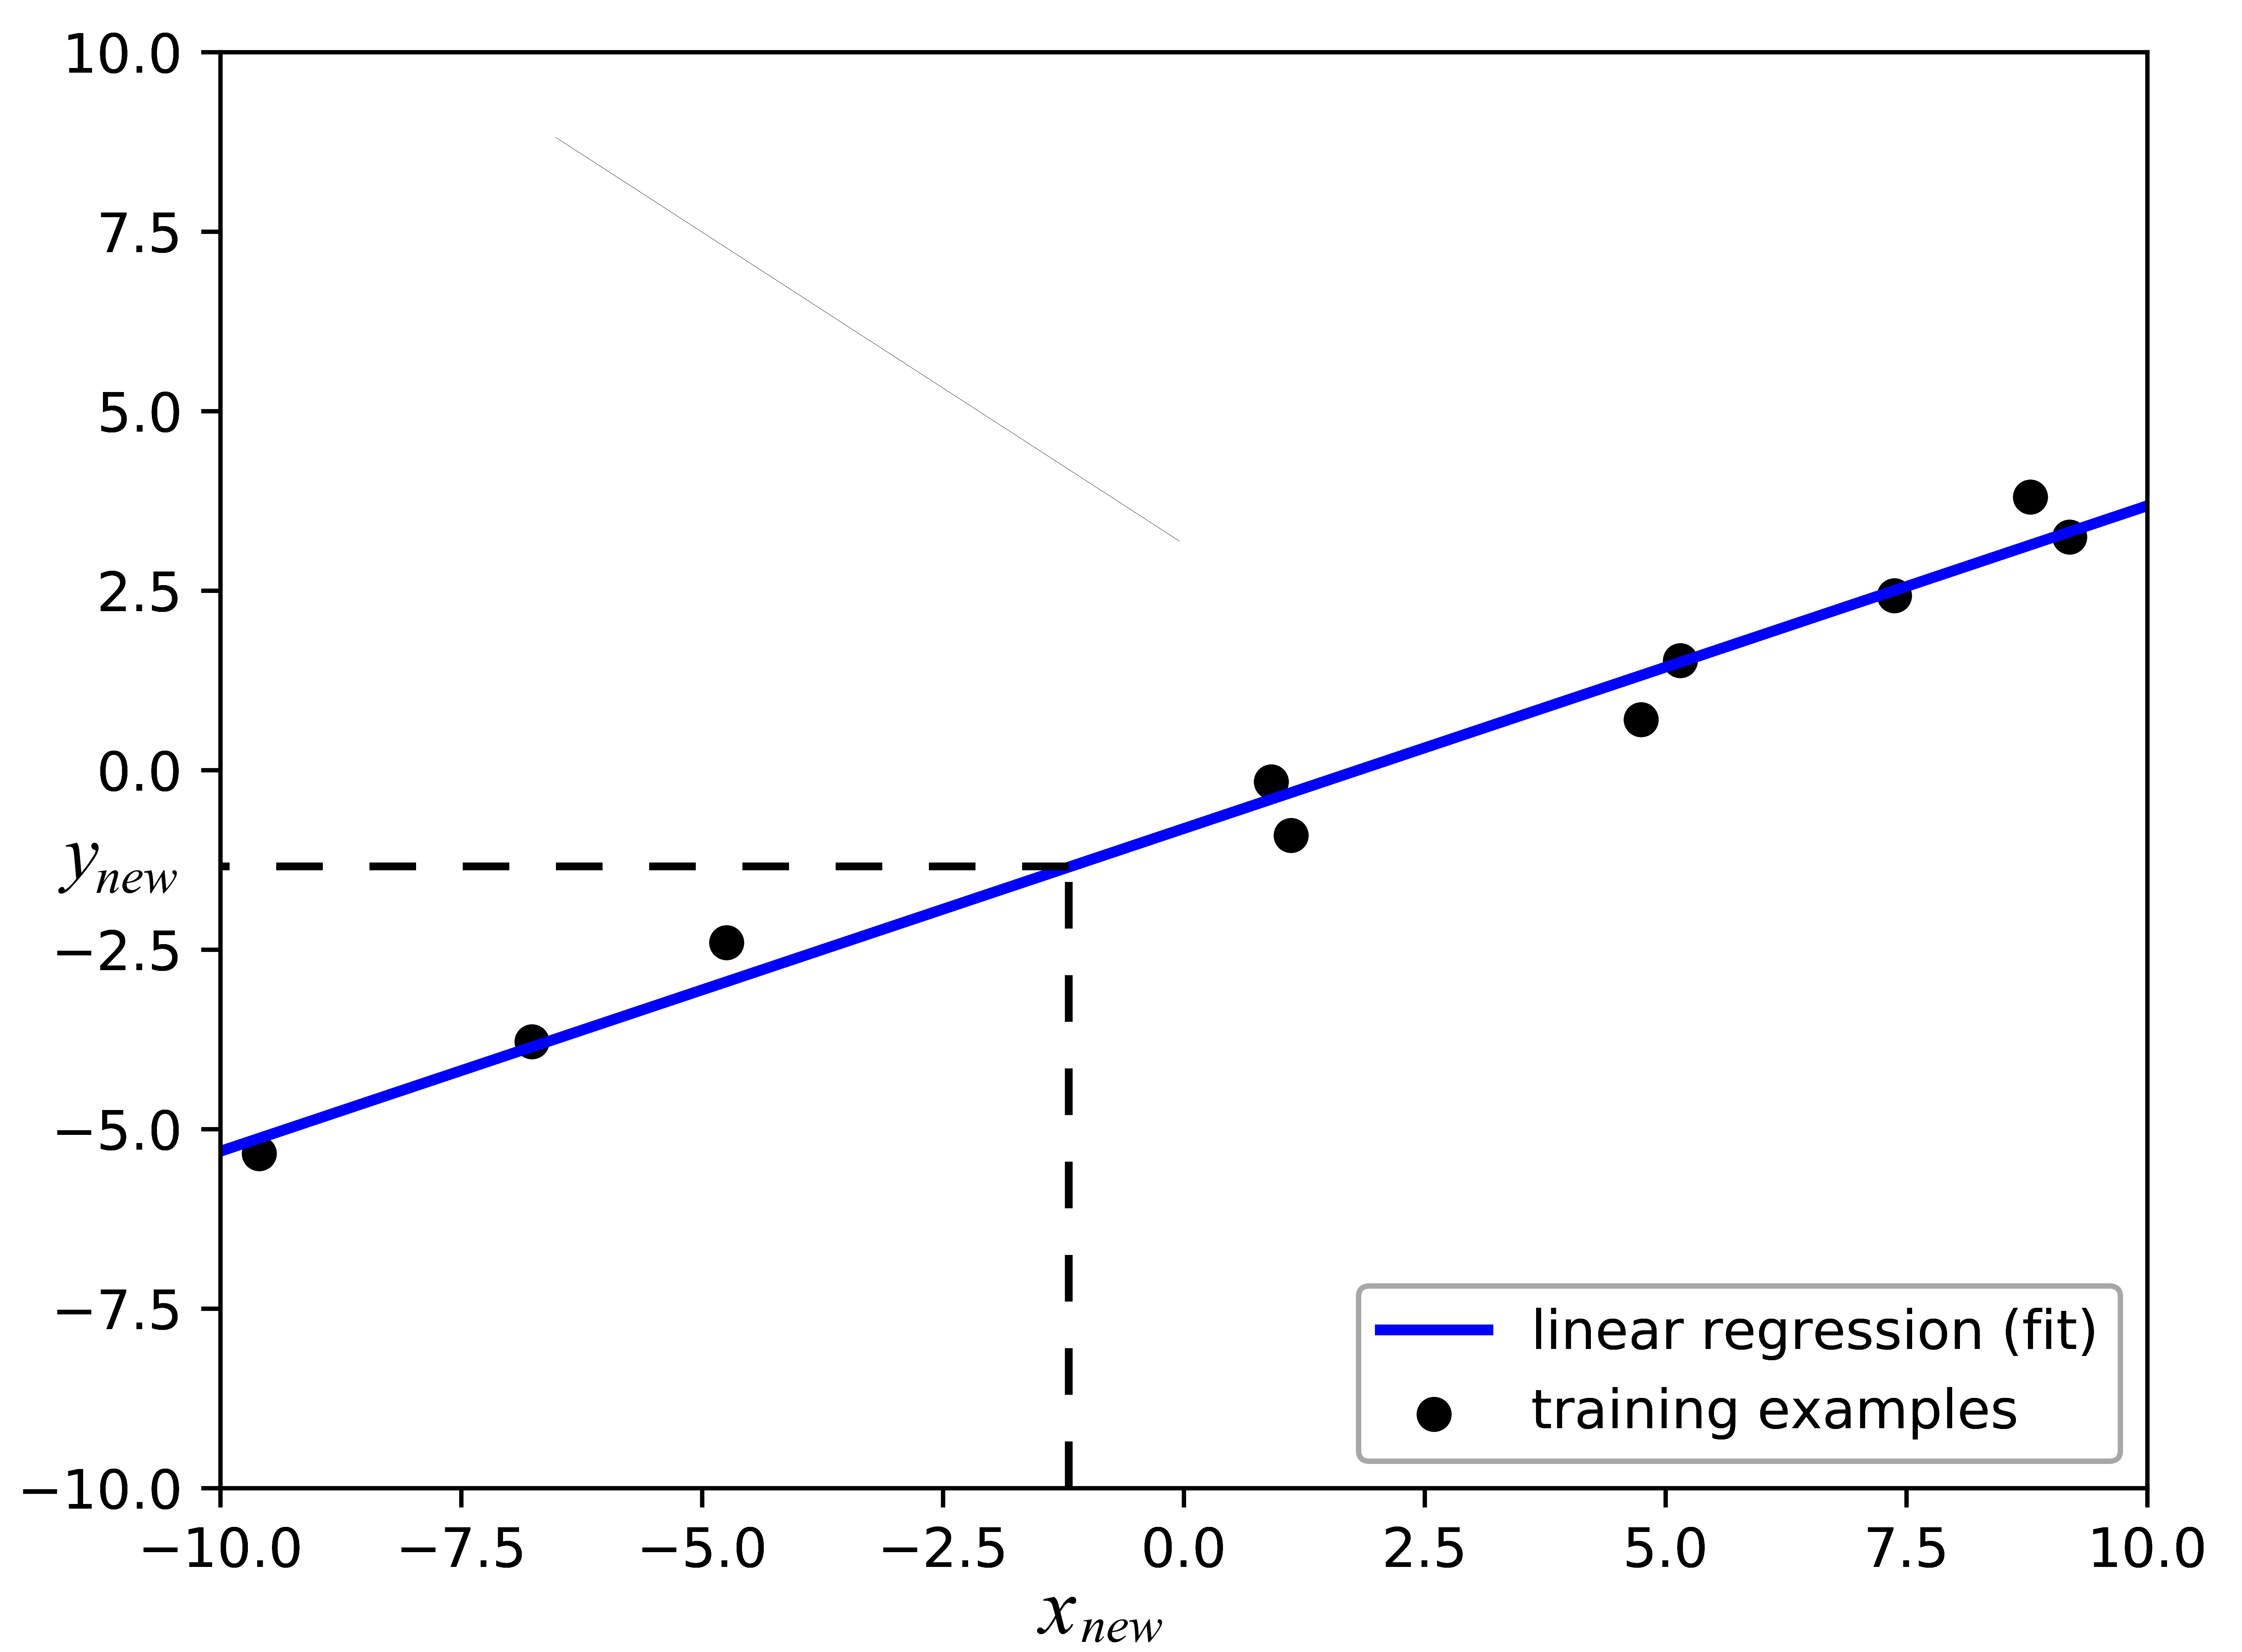
\includegraphics[width=1\textwidth,keepaspectratio]{Bilder/Linear_regression.png}};
	\end{tikzpicture}
	\urldef{\myurl}\url{https://alioh.github.io/images/2019-10-25/ch3-fig1.png}
	\caption[Lineare Regression]{Lineare Regression (Quelle: \protect\myurl{}, Zugriff 18.04.2024)}
	\label{fig: Lineare Regression}
\end{figure}

Lineare Modelle sind nicht nur auf eine Dimension beschränkt, sondern können auch in mehrdimensionalen Räumen angewandt werden, wo die Gleichung zu \(y = w_1x_1 + w_2x_2 + \ldots + w_nx_n + b\) erweitert wird. Hierbei repräsentieren \(w_1, w_2, \ldots, w_n\) die Gewichte der unabhängigen Variablen, was eine Modellierung komplexerer Zusammenhänge zwischen den Variablen ermöglicht. Für jeden zusätzlichen Parameter wird eine zusätzliche Dimension im Raum hinzugefügt, was die Modellkomplexität erhöht.

\subsubsection{Entscheidungsbaum}\label{sec: Decision Tree}
Ein Entscheidungsbaum ist ein Modell, das Daten anhand eines baumartigen Graphen klassifiziert oder vorhersagt. Jeder Knoten im Baum entspricht einer Entscheidungsregel, und die Blätter des Baumes repräsentieren die Ergebnisse. Entscheidungsbäume finden häufig Anwendung in der Kreditbewertung und medizinischen Diagnostik.

Von einem Wurzelknoten ausgehend teilt sich der Baum in Zweige, die durch Entscheidungsregeln definiert sind. Überschreitet oder unterschreitet ein Merkmal einen bestimmten Schwellenwert, verzweigt sich der Baum entsprechend. Dieser Prozess setzt sich rekursiv fort, bis ein Blatt erreicht wird, das das Endergebnis darstellt.

\begin{figure}[H]
	\centering
	\begin{tikzpicture}
		\node [anchor=south west] (image) at (0,0) {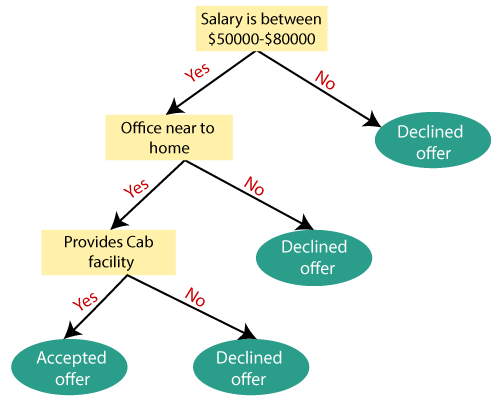
\includegraphics[width=0.8\textwidth,keepaspectratio]{Bilder/Decision_Tree.png}};
	\end{tikzpicture}
	\urldef{\myurl}\url{https://static.javatpoint.com/tutorial/machine-learning/images/decision-tree-classification-algorithm2.png}
	\caption[Entscheidungsbaum]{Entscheidungsbaum (Quelle: \protect\myurl{}, Zugriff 18.04.2024)}
	\label{fig: Decision Tree}
\end{figure}

\subsubsection{Random-Forest-Regressor}\label{sec: Random Forest Regressor}
Der Random-Forest-Regressor verwendet eine Ensemble-Methode, die mehrere Entscheidungsbäume während des Trainingsprozesses erstellt und die Vorhersagen dieser Bäume mittelt. Ensemble-Methoden funktionieren, indem sie die Vorhersagen mehrerer Modelle kombinieren, um die Genauigkeit zu verbessern. Diese Methode verbessert die Vorhersagegenauigkeit und reduziert die Gefahr der Überanpassung, weil jedes Modell unabhängig voneinander trainiert wird und somit unterschiedliche Fehler aufweist. Anwendung findet der Random-Forest-Regressor unter anderem bei der Vorhersage von Immobilienpreisen und Aktienmarktentwicklungen.

Wie bereits im \autoref{sec: Decision Tree} beschrieben, besteht ein Entscheidungsbaum aus mehreren Entscheidungsregeln, die zu einem Endergebnis führen. Der Random-Forest-Regressor baut auf einer Vielzahl solcher Bäume auf, die unabhängig voneinander auf zufälligen Teilmengen des Datensatzes trainiert werden, um die Variabilität zu reduzieren. Die finale Vorhersage ergibt sich aus der Mittelung der einzelnen Baumvorhersagen.

\begin{figure}[H]
    \centering
    \begin{tikzpicture}
        \node [anchor=south west] (image) at (0,0) {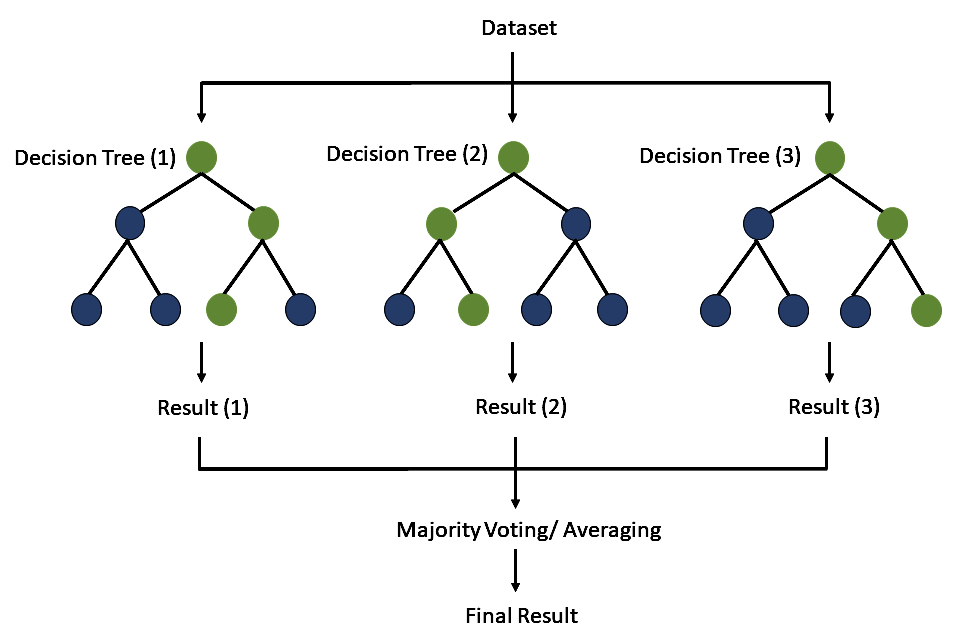
\includegraphics[width=1\textwidth,keepaspectratio]{Bilder/Random_forest.png}};
    \end{tikzpicture}
    \urldef{\myurl}\url{https://miro.medium.com/v2/resize:fit:720/format:webp/1*R3oJiyaQwyLUyLZL-scDpw.png}
    \caption[Random Forest]{Random Forest (Quelle: \protect\myurl{}, Zugriff 18.04.2024)}
    \label{fig: Random Forest}
\end{figure}

Der Prozess der Vorhersage mit einem Random-Forest-Regressor wird in \autoref{fig: Random Forest} veranschaulicht, wo mehrere Entscheidungsbäume dargestellt sind, die unabhängig voneinander trainiert werden. Die Gesamtvorhersage resultiert aus der Durchschnittsbildung der Vorhersagen dieser Bäume.

\subsubsection{Gradient-Boosting-Regressor}
Das Gradient-Boosting ist eine weitere fortgeschrittenere Ensemble-Technik, die sequenziell Modelle aufbaut, wobei jedes nachfolgende Modell versucht, die Fehler des vorherigen Modells zu korrigieren. Häufig wird dieses Verfahren zur Erstellung robuster Vorhersagemodelle in der Finanzwirtschaft und Biotechnologie eingesetzt.

Im Gegensatz zum Random Forest, bei dem die Bäume unabhängig voneinander trainiert werden, erfolgt das Training der Bäume beim Gradient Boosting sequenziell. Das anfängliche Modell, das die Daten schlecht vorhersagt, wird kontinuierlich durch Hinzufügen neuer Modelle verbessert, die jeweils die verbleibenden Fehler korrigieren. Dieser Prozess wird so lange fortgesetzt, bis ein vordefiniertes Kriterium erreicht ist.

\begin{figure}[H]
    \centering
    \begin{tikzpicture}
        \node [anchor=south west] (image) at (0,0) {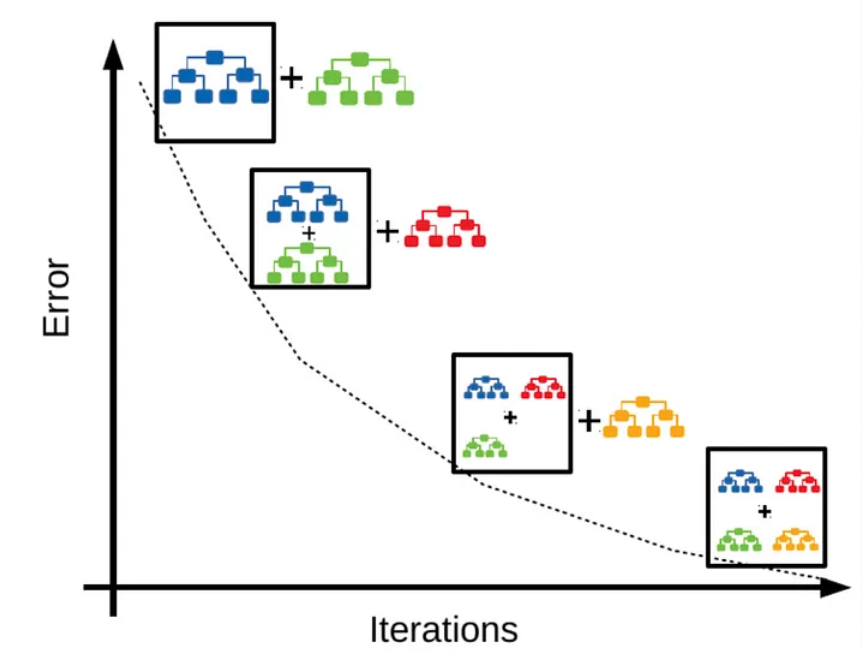
\includegraphics[width=0.8\textwidth,keepaspectratio]{Bilder/Gradient_Boosting.png}};
    \end{tikzpicture}
    \urldef{\myurl}\url{https://miro.medium.com/v2/resize:fit:720/format:webp/1*OZPOQUKiaVmZOEMm_-8iYA.png}
    \caption[Gradient Boosting]{Gradient Boosting (Quelle: \protect\myurl{}, Zugriff 18.04.2024)}
    \label{fig: Gradient Boosting}
\end{figure}

\autoref{fig: Gradient Boosting} zeigt, wie der Fehler in jedem Schritt der Iteration durch das Hinzufügen eines neuen Modells, das die Fehler des vorherigen Modells korrigiert, reduziert wird. Die Berechnung wird dadurch sehr rechenintensiv, aber die Genauigkeit der Vorhersagen wird verbessert.

\subsubsection{K-Nearest Neighbors Regressor}
Der K-Nearest Neighbors (KNN) Regressor basiert auf der Annahme, dass ähnliche Datenpunkte ähnliche Ergebnisse liefern. Dieses Modell wird zur Vorhersage von Werten neuer Datenpunkte eingesetzt und findet Anwendung in Bereichen wie Bilderkennung, Sprachverarbeitung und Finanzanalyse. Bei der Anwendung des KNN-Modells ist die Wahl der Anzahl von \(k\) Nachbarn sowie der Distanzmetrik entscheidend, da eine zu geringe Anzahl an Nachbarn zu einer Überanpassung und eine zu hohe Anzahl zu einer Unteranpassung führen kann.

\begin{figure}[H]
    \centering
    \begin{tikzpicture}
        \node [anchor=south west] (image) at (0,0) {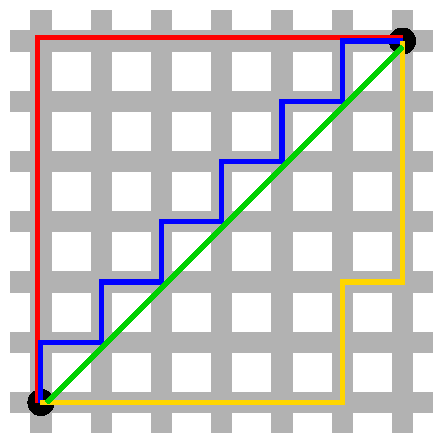
\includegraphics[width=0.6\textwidth,keepaspectratio]{Bilder/Manhattan_distance.pdf}};
    \end{tikzpicture}
    \urldef{\myurl}\url{https://de.wikipedia.org/wiki/Manhattan-Metrik#/media/Datei:Manhattan_distance.svg}
    \caption[Manhatten vs. Euklidischer Abstand]{Manhatten (rot, blau, gelb) vs. Euklidischer (grün)Abstand (Quelle: \protect\myurl{}, Zugriff 30.04.2024)}
    \label{fig: Manhattan}
\end{figure}

Der Prozess des KNN-Modells umfasst drei Schritte:
\begin{enumerate}
    \item Auswahl der Anzahl \(k\), der zu betrachtenden nächsten Nachbarn sowie Festlegung einer geeigneten Metrik zur Berechnung der Distanz zwischen den Datenpunkten, beispielsweise der euklidische oder der Manhattan-Abstand wie in \autoref{fig: Manhattan} zu sehen ist.
    \item Ermittlung der \(k\) nächstgelegenen Nachbarn des zu klassifizierenden Datenpunkts durch Berechnung der Distanzen zu allen anderen Datenpunkten. Die \(k\) Datenpunkte mit der geringsten Distanz werden ausgewählt.
    \item Zuweisung einer Klassenbezeichnung zum zu klassifizierenden Datenpunkt durch eine Mehrheitsabstimmung unter den \(k\) nächsten Nachbarn. Die am häufigsten vorkommende Klasse unter den \(k\) Nachbarn wird als Vorhersage für den zu klassifizierenden Datenpunkt verwendet.
\end{enumerate}

\begin{figure}[H]
    \centering
    \begin{tikzpicture}
        \node [anchor=south west] (image) at (0,0) {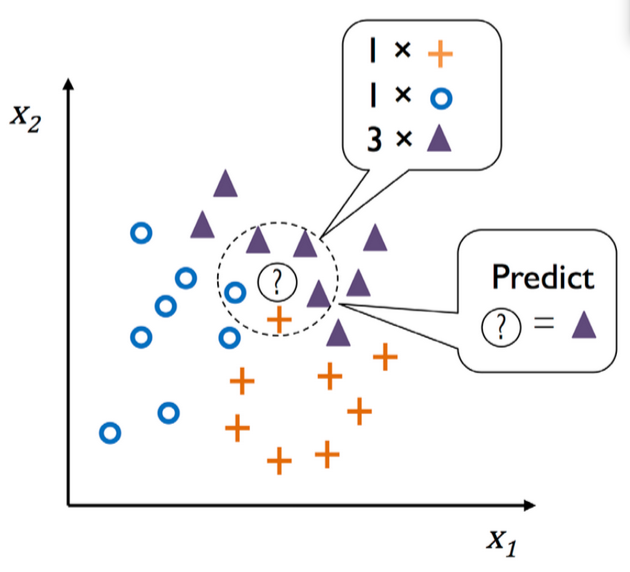
\includegraphics[width=0.8\textwidth,keepaspectratio]{Bilder/k_nearest.png}};
    \end{tikzpicture}
    \caption[K-Nearest Neighbors]{K-Nearest Neighbors (Quelle: \cite[][Seite 99]{raschkaMachineLearningPyTorch2022})}
    \label{fig: K-Nearest Neighbors}
\end{figure}

\autoref{fig: K-Nearest Neighbors} veranschaulicht ein Beispiel für den K-Nearest Neighbors-Ansatz, bei dem die Klassenzugehörigkeit eines Datenpunkts basierend auf den \(k\) nächstgelegenen Nachbarn bestimmt wird. In diesem Fall ist \(k = 5\), und die Klassenzugehörigkeit des Datenpunkts wird durch eine Mehrheitsentscheidung der fünf nächsten Nachbarn bestimmt, wobei das lilafarbene Dreieck am häufigsten vorkommt und daher als Vorhersage für den zu klassifizierenden Datenpunkt verwendet wird.

\subsubsection{Neuronales Netzwerk Regressor}
Der neuronale Netzwerk-Regressor ist ein Modell, das auf der Struktur des menschlichen Gehirns basiert und künstliche Neuronen verwendet, um komplexe Beziehungen zwischen Variablen zu modellieren. Einsatzgebiete dieses Modells umfassen die Bilderkennung, Sprachverarbeitung und Finanzanalyse.

Ein künstliches neuronales Netzwerk besteht aus mehreren Schichten von Neuronen, die miteinander verbunden sind. Jedes Neuron erhält Eingaben von anderen Neuronen, führt eine Berechnung durch und gibt das Ergebnis weiter. Die Neuronen sind in Schichten organisiert: Die Eingabeschicht nimmt die Eingangsdaten auf, während die Ausgabeschicht die Vorhersage liefert und die verborgenen Schichten die komplexen Beziehungen zwischen den Variablen modellieren.

\begin{figure}[H]
    \centering
    \begin{tikzpicture}
        \node [anchor=south west] (image) at (0,0) {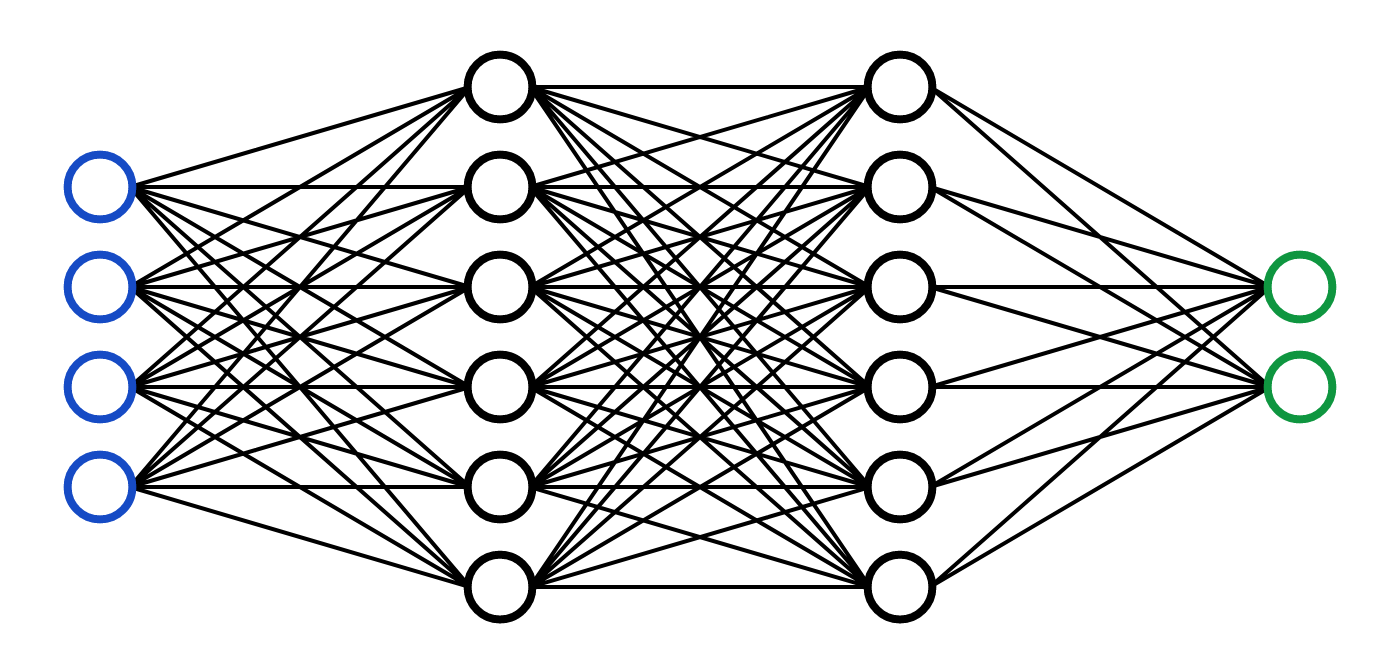
\includegraphics[width=1\textwidth,keepaspectratio]{Bilder/neural_network.png}};
    \end{tikzpicture}
    \urldef{\myurl}\url{https://victorzhou.com/media/nn-series/network.svg}
    \caption[Neuronales Netzwerk]{Neuronales Netzwerk (Quelle: \protect\myurl{}, Zugriff 18.04.2024)}
    \label{fig: Neural Network}
\end{figure}

\autoref{fig: Neural Network} zeigt ein Beispiel für ein künstliches neuronales Netzwerk mit einer Eingabeschicht, zwei verborgenen Schichten und einer Ausgabeschicht. Die Eingabeschicht nimmt die Daten auf, die verborgenen Schichten verarbeiten die Daten, indem sie die komplexen Beziehungen zwischen den Variablen modellieren, und die Ausgabeschicht liefert die Vorhersage des Modells.

\subsubsection{Support Vector Machine Regressor}\label{sec: Support Vector Machine Regressor}
Die Support Vector Machine (SVM) ist ein Regressions- und Klassifikationsmodell, das darauf abzielt, eine Hyperplane (Trennlinie) zu finden, welche die größtmögliche Trennung zwischen zwei Klassen von Datenpunkten erreicht. Dieses Modell wird in der Bilderkennung, Textklassifizierung und Finanzanalyse eingesetzt.

Die SVM arbeitet, indem sie die Hyperplane zwischen zwei Klassen von Datenpunkten findet, die den größtmöglichen Abstand zwischen den Klassen aufweist. Die SVM maximiert diesen Abstand, um die Genauigkeit der Klassifizierung zu verbessern, und kann sowohl für lineare als auch für nicht-lineare Daten eingesetzt werden, was sie von der linearen Regression unterscheidet.

\begin{figure}[H]
\begin{subfigure}[c]{0.5\textwidth}
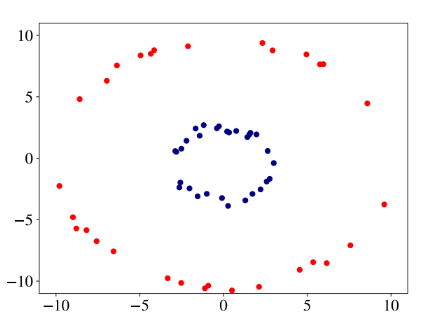
\includegraphics[width=\textwidth]{Bilder/before_svm.png}
\end{subfigure}
\begin{subfigure}[c]{0.5\textwidth}
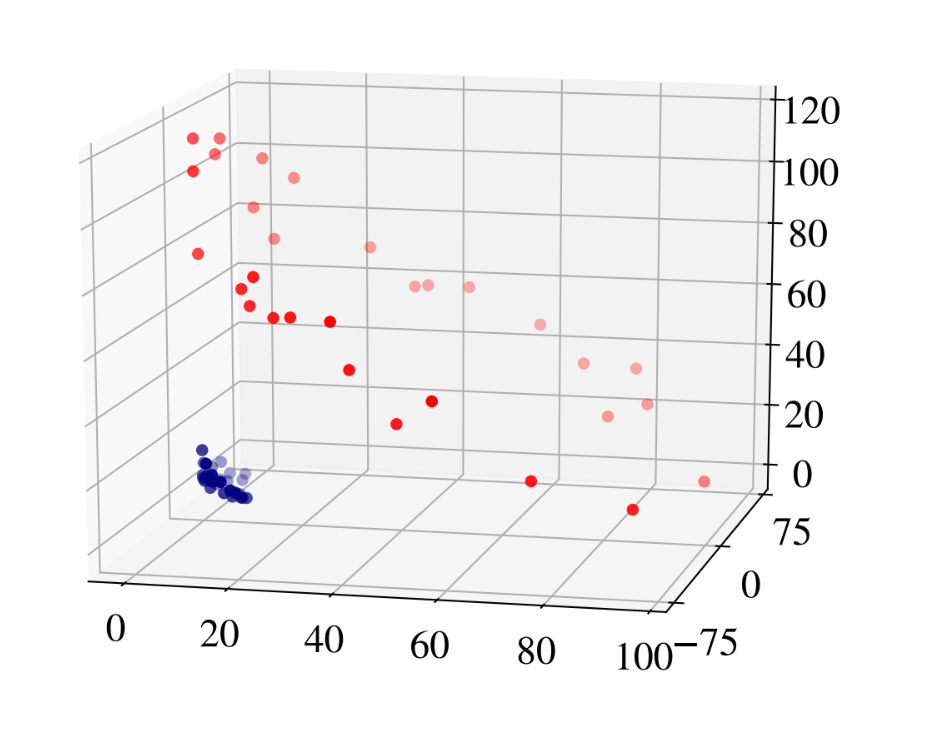
\includegraphics[width=\textwidth]{Bilder/SVM.png}
\end{subfigure}

\caption[Support Vector Machine]{Support Vector Machine (Quelle: \cite[vgl.][Kapitel: Fundamental Algorithms, Seite 12-14]{burkov2019hundred})}
    \label{fig: Support Vector Machine}
\end{figure}

Wie in \autoref{fig: Support Vector Machine} dargestellt, ermöglicht die SVM die Trennung von Daten, die im zweidimensionalen Raum nicht separierbar sind. Die Daten im linken Bild sind durch eine Linie oder Ebene nicht trennbar. Indem sie in einen höherdimensionalen Raum projiziert werden, was im rechten Bild zu sehen ist, wird eine lineare Trennung möglich.

\subsection{Benchmarks}\label{sec: Benchmarks}
Benchmarks werden genutzt, um ähnliche Produkte oder Software miteinander zu vergleichen. Bei Computerprogrammen wird oft die Laufzeit oder die Genauigkeit der Vorhersagen gemessen. In dieser Arbeit werden Benchmarks eingesetzt, um die Genauigkeit der Modelle zu bewerten.

\subsubsection{Mean Squared Error (MSE)}
Der Mean Squared Error (MSE) ist der am häufigsten verwendete Benchmark zur Bewertung von Machine-Learning-Modellen. Die Formel für den MSE lautet:

\begin{align}
\textit{MSE} &= \frac{1}{n} \sum_{i=1}^{n} (y_i - \hat{y}_i)^2\\
n &= \textit{Anzahl der Datenpunkte}\\
y_i &= \textit{Beobachtete Werte}\\
\hat{y}_i &= \textit{Vorhergesagte Werte}
\end{align}

\subsubsection{R2-Score}
Der R2-Score misst die Genauigkeit eines Modells im Vergleich zu einem einfachen Durchschnittsmodell. Die Formel hierzu lautet:

\begin{equation}
\textit{R2-Score} = 1 - \frac{\sum_{i=1}^{n} (y_i - \hat{y}_i)^2}{\sum_{i=1}^{n} (y_i - \bar{y})^2}
\end{equation}

Der R2-Score variiert zwischen 0 und 1, wobei ein Wert von 1 eine perfekte Vorhersage und ein Wert von 0 keine Vorhersagekraft des Modells bedeutet.

\subsubsection{Vergleichsstrategie in diesem Projekt}
Für den Vergleich der Modelle wird eine umfassende Tabelle erstellt, in der jede Spalte einem Modell entspricht. In den Zeilen stehen verschiedene Konfigurationen oder Datenverarbeitungsschritte. In den Zellen befinden sich die Benchmarks (Mean Squared Error und R2-Score). Am Ende der Analyse können die Zellen farblich markiert sowie Durchschnitte berechnet werden, um festzustellen, welches Modell insgesamt am besten abschneidet.

\subsection{Datenverarbeitung}\label{sec: Data Preprocessing}
Die Datenverarbeitung bezieht sich auf die vorbereitenden Schritte, die notwendig sind, um Rohdaten in ein Format zu überführen, das effektiv von Datenanalysesystemen oder Machine-Learning-Algorithmen verarbeitet werden kann. Dieser Prozess ist entscheidend, da er die Qualität und Effektivität der Datenanalyse und Modellvorhersagen verbessert.

Im Rahmen dieses Projekts wurden kontinuierlich weitere Datenverarbeitungsschritte integriert, um die Datenqualität zu erhöhen. Zu diesen Schritten gehören unter anderem das Entfernen von fehlenden Werten, das Skalieren der Daten, das Kodieren von kategorialen Variablen und das Aufteilen der Daten in Trainings- und Testsets.

\subsection{Hyperparameter-Tuning}\label{sec: Hyperparameter Tuning}
Hyperparameter-Tuning ist der Prozess der Optimierung der Parameter, die die Konfiguration eines Machine-Learning-Modells steuern. Ziel ist es, die beste Kombination von Parametern zu finden, die die Leistung des Modells maximiert. Zu den Methoden des Hyperparameter-Tunings gehören unter anderem Optuna, eine Bibliothek für automatische Hyperparameter-Optimierung, und Randomized Grid Search, eine Technik, die eine zufällige Auswahl von Parametern aus einer definierten Liste testet, um effizient optimale Modelleinstellungen zu identifizieren.

\subsubsection{Optuna}\label{sec: Optuna}
Optuna ist eine Bibliothek für automatische Hyperparameter-Optimierung, die Bayesian Optimization verwendet, um die besten Hyperparameter für ein Modell zu finden. In diesem Projekt wird Optuna genutzt, um den optimalen Schwellenwert für Kauf- oder Verkaufsentscheidungen zu bestimmen.

\subsubsection{Randomized Grid Search}\label{sec: Randomized Grid Search}
Randomized Grid Search ist eine Technik, die eine zufällige Auswahl von Parametern aus einer definierten Liste testet, um effizient die besten Hyperparameter für ein Modell zu finden. In diesem Projekt wurde eine JSON-Datei erstellt, die alle zu testenden Parameter für die in \nameref*{sec: Machine Learning Modelle} aufgeführten Modelle enthält. Die Bibliothek führt dann eine Reihe von Tests durch und gibt die optimalen Parameter zurück.\\
\autoref{fig: Randomized Grid Search} zeigt eine Visualisierung des Randomized Grid Search-Prozesses. In dem vereinfachten Fall werden nur zwei Parameter getestet, um die optimale Kombination zu finden.
Der grüne Punkt zeigt die optimale Kombination der Parameter, die den besten Score erzielt hat.
\begin{figure}[H]
    \centering
    \begin{tikzpicture}
        \node [anchor=south west] (image) at (0,0) {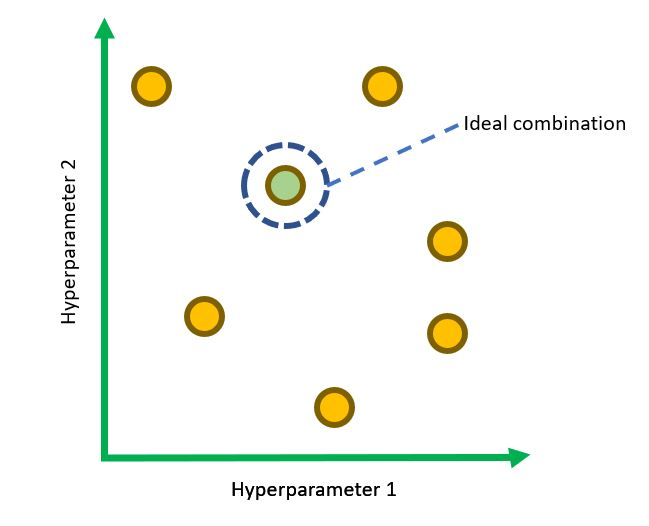
\includegraphics[width=0.8\textwidth,keepaspectratio]{Bilder/randomized_search.jpeg}};
    \end{tikzpicture}
    \urldef{\myurl}\url{https://editor.analyticsvidhya.com/uploads/72089randomized.JPG}
    \caption[Randomized Grid Search]{Randomized Grid Search (Quelle: \protect\myurl{}, Zugriff 30.04.2024)}
    \label{fig: Randomized Grid Search}
\end{figure}

\subsection{Methodik}\label{sec: Methodik}
In einem Programmierprojekt ist es wesentlich, nicht nur den Code zu schreiben, sondern auch eine Methode zu haben, um die Ergebnisse zu überprüfen und zu vergleichen.

Wie in \nameref{sec: Benchmarks} erläutert, werden zwei Benchmarks verwendet, um die Modelle zu vergleichen: der Mean Squared Error und der R2-Score. Aus diesen beiden Benchmarks wird ein Gesamtscore berechnet, indem der R2-Score invertiert wird, sodass ein kleinerer Wert besser ist als ein größerer. Dazu werden alle Werte von 1 abgezogen, sodass ein Score von 0.7 zu einem Score von 0.3 wird.

Im nächsten Schritt werden der Mean Squared Error und der invertierte R2-Score multipliziert, um den Gesamtscore zu erhalten. Die Formel für den Gesamtscore lautet:

\begin{equation}
    \textit{Gesamtscore} = (1 - \textit{R2}) \cdot \textit{MSE}
\end{equation}

Die Vorhersagequalität wird iterativ verbessert, indem einzelne Datenverarbeitungsschritte aufeinander aufbauen. Diese Schritte werden anhand des Gesamtscores gemessen. Dieser wird zusammen mit einer Beschreibung der durchgeführten Änderungen in einer Tabelle festgehalten. Die Tabelle enthält alle Modelle und die Scores für die verschiedenen Schritte. Am Ende wird der Durchschnitt der Scores berechnet, um zu ermitteln, welches Modell insgesamt am besten abgeschnitten hat. Des Weiteren lässt sich so auch feststellen, welche Schritte die größte Verbesserung gebracht haben und wie die einzelnen Modelle auf die Schritte reagiert haben.